\chapter{Methodology}\label{ch:methodology}

Following is a short overview of methodologies applied during crucial steps in our process that will be discussed in more detail in the following sections:

\begin{enumerate}
    \item Preparation
    \begin{itemize}
        \item Selection of \gls{Blockchain} network
        \item Selection of technology stack
        \item Architectural design
    \end{itemize}
    \item Development
    \begin{itemize}
        \item Versioning
        \item Agile development
        \item End-to-end tests
    \end{itemize}
    \item Evaluation
    \begin{itemize}
        \item Test analysis
        \item Technical analysis
        \item Cryptocurrency transaction analysis
    \end{itemize}
\end{enumerate}

\section{Preparation}\label{sec:preparation}

\subsection{Selection of blockchain network}\label{subsec:selection-of-blockchain-network}

As seen in \cref{tab:selection-of-blockchain-network}, the findings in~\cref{sec:voting-systems} can be applied as selection criteria for relevant \gls{Blockchain} networks (see \cref{subsec:comparison-of-turing-complete-blockchains}).
However, some properties mentioned in~\cref{sec:voting-systems} depend entirely on decisions relating to frontend design and code governance rather than the selected \gls{Blockchain}, e.g., whether the software is open-source.
These are displayed in gray in~\cref{tab:selection-of-blockchain-network}.

\begin{table}[t]
    \begin{tabularx}{\textwidth}{bCCCC}
        \hline
        \textbf{Property} & \textbf{Ethereum} & \textbf{Hyperledger Fabric} & \textbf{Polygon} & \textbf{Solana} \\
        \hline
        Auditability & \dblcmark & \dblcmark & \dblcmark & \dblcmark \\
        \hline
        Anonymity & \dblcmark & \cmark & \dblcmark & \cmark  \\
        \hline
        \rowcolor{lightgray}
        Usability & - & - & - & -  \\
        \hline
        \rowcolor{lightgray}
        Accessibility & - & - & - & - \\
        \hline
        Security & \dblcmark & \cmark & \dblcmark & \cmark   \\
        \hline
        Scalability & \xmark & \cmark & \cmark & \cmark  \\
        \hline
        \rowcolor{lightgray}
        Transparency & - & - & - & - \\
        \hline
        Incoercibility & \xmark & \xmark & \xmark & \xmark  \\
        \hline
    \end{tabularx}
    \caption[Potential blockchain networks]{Potential blockchain networks}
    \label{tab:selection-of-blockchain-network}
\end{table}

All four \gls{Blockchain} networks possess most of the properties mentioned in~\cref{sec:voting-systems}.
Nevertheless, as shown in \cref{subsec:comparison-of-turing-complete-blockchains}, scalability seems to be a major issue underlying \gls{Blockchain} technology in general.
For instance, even though the Ethereum Foundation is looking to improve Ethereum's protocol further, theoretically enabling it to process up to 100,000 \gls{TPS} in the future, as of the time of this writing, it is not able to process enough transactions to facilitate national elections.
Conversely, other \glspl{Blockchain} compromise on similarly essential features like security or network stability, an equally important scalability aspect, to achieve a higher number of \gls{TPS}.
Unfortunately, in the absence of a \gls{Blockchain} protocol that satisfies all aspects shown in~\cref{sec:voting-systems}, compromises in our selection process were unavoidable.
With this in mind and looking at \cref{tab:selection-of-blockchain-network}, Polygon seemed to be the most logical choice as it runs on top of Ethereum.
Therefore, it automatically benefits from Ethereum's superior security and anonymity, as well as all future improvements made to Ethereum's protocol, while still giving it an edge in terms of scalability due to its Layer 2 protocol (see~\cref{subsec:comparison-of-turing-complete-blockchains}).

\subsection{Selection of technology stack}\label{subsec:selection-of-tech-stack}

There are certainly many frameworks that could be used to develop the server- and client-side of a decentralized electronic voting system.
However, we relied on a full Node.js integration due to its non-blocking \gls{IO} to ensure high scalability (see~\cref{subsec:node.js}).
Similarly, given the scalability advantages of monorepos (see~\cref{subsec:nx}), we utilized nx to manage the project's repository.
Additionally, keeping transparency in mind (see~\cref{sec:voting-systems}), an open-source project built with nx is more accessible to other developers as a resource for future research.

We used Next.js as a framework on the client side as it allows for server-side rendering, increasing the application's overall security (see~\cref{subsec:next.js}) and making it \glstext{SEO}-friendly.
Alternatively, we could have developed the client-side with Nuxt.js, which mimics most of Next.js's server-side and static rendering methods while using Vue.js instead of React.js under the hood.
Nevertheless, Nuxt.js has a smaller community, arguably making React.js the preferable choice.

Although Next.js comes with its own routing framework for API calls, it is reasonable to use a separate framework for requests that handle database and smart contract actions.
Therefore, we utilized Nest.js, which eased the process of following best practices for developing backend applications.
As illustrated in~\cref{subsec:nest.js}, Nest.js is specifically designed with scalability in mind;
moreover, it ensures high readability for developers with either an \gls{OOP} or \gls{FP} background.
Likewise, we handled database-related aspects of the application using a PostgreSQL database since a broad spectrum of developers should be familiar with a \gls{ORDBMS} and PostgreSQL in particular (see~\cref{subsec:postgresql}).

\subsection{Architectural design}\label{subsec:architectural-design}


\section{Development}\label{sec:development}

\subsection{Versioning}\label{subsec:versioning}

We used Git Workflows to version the project during development, which enabled parallel workflows depending on features and provided greater flexibility.
Furthermore, it enabled the analysis of code changes during our iterative process and revision of changes and is well-established in the software industry and does not have serious contenders that are also open-source.

\subsection{Agile development}\label{subsec:agile-development}

The development methods displayed in \cref{fig:success-rates-development-methods} are sorted according to their success rates.
As stated by~\textcite[10-12]{jones_software_2010}, projects with a size of less than 1000 function points are most likely to benefit from agile development methods.
The median size of function points is defined as 53 lines of JavaScript code by~\textcite{qsm_function_2009}.
Based on these findings, we applied agile development methods during the development process as the project's size was not anticipated to grow beyond the aforementioned dimensions.

However, we departed from the recommended defect prevention methods shown in~\cref{fig:success-rates-development-methods} since embedded user reviews mainly test the application’s frontend functionality.
Instead, the same goal could be achieved by applying Scrum methods and \gls{E2E} tests.

\begin{figure}[t]
    \begin{subfigure}[b]{\textwidth}
        \centering
        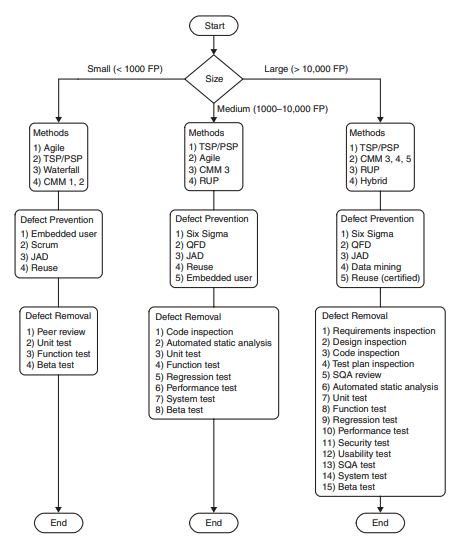
\includegraphics[width=0.7\textwidth]{jones-2010-development-methods}
        \caption[Success rates of development methods]{Success rates of development methods in relation to project size~\autocite[11]{jones_software_2010}}
        \label{fig:success-rates-development-methods}
    \end{subfigure}
    \begin{subfigure}[b]{\textwidth}
        \centering
        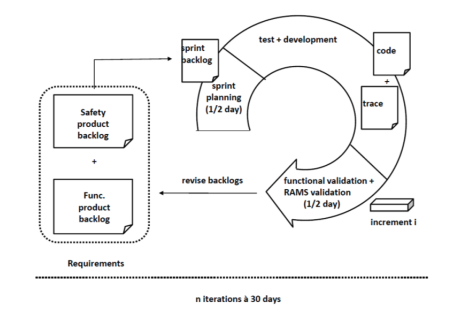
\includegraphics[scale=.8]{myklebust-2014-scrum}
        \caption[Scrum method]{Scrum method~\autocite[2]{myklebust_scrum_nodate}}
        \label{fig:scrum-method}
    \end{subfigure}
    \caption{Development methods}\label{fig:development-methods}
\end{figure}

\subsection{Personal Scrum}\label{subsec:personal-scrum}

Despite this being a one-person project with different organizational requirements than projects developed by a team, we applied scrum methods during our development process.
As stated by \textcites{andrews_scrum_2017}{pahuja_scrum_2015}, this meant adapting scrum methods for personal use, enabling us to establish iterative processes to track the development process, evaluate intermediate results and remove defects (see~\cref{fig:scrum-method}).

\subsection{End-to-end tests}\label{subsec:end-to-end-tests}

Since peer reviews are no feasible option for defect removal in a single-person project, we employed E2E tests to check the application’s intended functionality and iteratively remove possible defects.
Also, in contrast to unit tests, \gls{E2E} tests provided the possibility to test entire workflows of the application, such as the registration or voting process.

\section{Evaluation}\label{sec:evaluation}

The primary objective of this thesis was the development of a decentralized voting system under the assumption that such a system would dramatically improve upon fundamental properties of voting systems compared to analogous and centralized electronic systems.
For this, we first identified objectives based on a qualitative analysis of relevant research data (see~\cref{sec:voting-systems}) and quantified established \gls{E2E} election processes of analogous voting systems to convert them into software features mirroring the process.


\subsection{Tests}\label{subsec:tests}
\subsection{Cryptocurrency transaction analysis}\label{subsec:crypto-currency-transaction-analysis}